\documentclass[conference]{IEEEtran}
\IEEEoverridecommandlockouts
\usepackage{cite}
\usepackage{amsmath,amssymb,amsfonts}
\usepackage{algorithmic}
\usepackage{graphicx}
\usepackage{textcomp}
\usepackage{xcolor}
\usepackage[utf8]{inputenc}
\usepackage[T1]{fontenc}
\usepackage[turkish]{babel}

\def\BibTeX{{\rm B\kern-.05em{\sc i\kern-.025em b}\kern-.08em
    T\kern-.1667em\lower.7ex\hbox{E}\kern-.125emX}}
    
\begin{document}

\title{Büyük Ölçekli Sırt Çantası (Knapsack) Problemlerinde Genetik Algoritma ile Dinamik Programlamanın Başarım ve Zaman Karmaşıklığı Karşılaştırması}

\author{\IEEEauthorblockN{Hasan Yiğit Akbulut}
\IEEEauthorblockA{\textit{Yazılım Mühendisliği Bölümü} \\
\textit{Manisa Celal Bayar Üniversitesi}\\
Manisa, Türkiye \\
232802046@ogr.cbu.edu.tr}
\and
\IEEEauthorblockN{Erva Dal}
\IEEEauthorblockA{\textit{Yazılım Mühendisliği Bölümü} \\
\textit{Manisa Celal Bayar Üniversitesi}\\
Manisa, Türkiye \\
232803021@ogr.cbu.edu.tr}
\and
\IEEEauthorblockN{Beyda Coşkuner}
\IEEEauthorblockA{\textit{Yazılım Mühendisliği Bölümü} \\
\textit{Manisa Celal Bayar Üniversitesi}\\
Manisa, Türkiye \\
232803036@ogr.cbu.edu.tr}
}
\maketitle

\begin{abstract}
Bu bildiride, NP-Hard sınıfında yer alan Sırt Çantası (Knapsack) probleminin çözümünde, kesin sonuç (exact) üreten Dinamik Programlama (DP) ile sezgisel (heuristic) yaklaşım sunan Genetik Algoritma (GA) yöntemlerinin performansları karşılaştırılmıştır. Artan veri boyutları (N=100, N=1000 ve N=10000) altında algoritmaların zaman karmaşıklıkları ve optimum değerden sapma oranları deneysel olarak incelenmiştir. Test sonuçlarına göre, N=10000 elemanlı veri setinde DP algoritması 990.48 saniyede kesin optimuma ulaşırken, GA ayni problemi 1.02 saniyede yuzde 65.12 sapma orani ile çözmüştür. Ayrica, kesin kapasite kısıtlarına sahip problemlerde GA'nın esnek ceza fonksiyonlarına karşı duyarlılığı tartışılmıştır.
\end{abstract}

\begin{IEEEkeywords}
Knapsack Problemi, Dinamik Programlama, Genetik Algoritma, NP-Hard, Zaman Karmaşıklığı
\end{IEEEkeywords}

\section{Giriş (Introduction)}
Kombinatoryal optimizasyon alanındaki en temel NP-Hard problemlerinden biri olan Sırt Çantası (Knapsack) problemi, sınırlı bir kapasiteye sahip alana, toplam değeri maksimize edecek şekilde uygun eşyaların seçilmesi esasına dayanır. Problemin çözümünde Dinamik Programlama (DP) gibi kesin (exact) algoritmalar global optimumu garanti etse de, veri boyutu ($N$) ve kapasite kısıtı ($W$) arttıkça üstel olarak artan bir zaman ve alan karmaşıklığı sergilerler.

Bu çalışmanın temel amacı, DP algoritmasının sistem kaynaklarını tükettiği darboğaz noktalarını tespit etmek ve bu noktalarda Genetik Algoritma (GA) gibi evrimsel sezgisel yöntemlerin ne ölçüde hız kazandırdığını (ölçeklenebilirlik) ve optimumdan ne kadar saptığını (accuracy gap) ölçmektir.

\section{Literatür Taraması}
Literatürde Sırt Çantası problemi için uygulanan yöntemler temel olarak iki kategoriye ayrılır. Kesin çözüm yöntemleri (Dinamik Programlama, Dal-Sınır Algoritmaları) küçük ve orta ölçekli veri setlerinde başarı gösterirken; veri boyutu büyüdüğünde Genetik Algoritmalar, Karınca Kolonisi Optimizasyonu ve Tabu Arama gibi metasezgisel (metaheuristic) algoritmalar tercih edilmektedir \cite{b2}. Yakın dönem çalışmaları, sezgisel yöntemlerin kesin kapasite sınırlarına uyum sağlayabilmesi için özel onarım (repair) veya ceza (penalty) operatörlerine ihtiyaç duyduğunu göstermektedir \cite{b3}.

\section{Yöntem (Method)}

\subsection{Dinamik Programlama Yaklaşımı}
DP algoritması, problemi daha küçük alt problemlere bölerek çözer. Zaman ve alan karmaşıklığı $O(N \cdot W)$'dir. Durum geçiş denklemi şu şekilde tanımlanmıştır:
\begin{equation}
DP[i][w] = \max(v_i + DP[i-1][w-w_i], DP[i-1][w])\label{eq:dp}
\end{equation}
Burada $v_i$ eşyanın değerini, $w_i$ ağırlığını, $W$ ise anlık kapasiteyi temsil etmektedir.

\subsection{Genetik Algoritma Yaklaşımı}
GA, popülasyon tabanlı sezgisel bir aramadır. Bu çalışmada kromozomlar ikili (0-1) dizilimler olarak kodlanmıştır. Algoritma $O(N \cdot P \cdot G)$ zaman karmaşıklığına sahiptir ($P$: Popülasyon boyutu, $G$: Jenerasyon sayısı).

Kapasite kısıtını ($W$) aşan çözümleri elemek için esnek ceza (soft penalty) fonksiyonu uygulanmıştır:
\begin{equation}
Fitness = \sum (v_i \cdot x_i) - \max(0, \sum (w_i \cdot x_i) - W) \cdot 5\label{eq:ga}
\end{equation}

\section{Deneysel Sonuçlar (Experiments)}
Algoritmaların performansını ölçmek üzere $N=100$, $N=1000$ ve $N=10.000$ elemanlı sentetik veri setleri oluşturulmuştur. Çanta kapasitesi $W$, her veri setindeki toplam ağırlığın $\%30$'u olarak sabitlenmiştir. 

\subsection{Hesaplama Süreleri ve Doğruluk}
Tablo \ref{tab:performance}'de algoritmaların ulaştığı maksimum değerler ve çalışma süreleri sunulmuştur. N=100 ve N=1000 durumlarında GA'nın uyguladığı esnek ceza fonksiyonu yetersiz kalmış ve geçerli bir çözüm uzayı bulunamadığı için değer 0 olarak dönmüştür (sapma $\%100$). Ancak N=10.000 seviyesinde, GA geçerli bir sonuç üretmeyi başarmıştır. 

\begin{table}[htbp]
\caption{DP ve GA Performans Karşılaştırması}
\begin{center}
\begin{tabular}{|c|c|c|c|c|c|c|}
\hline
\textbf{N} & \textbf{Kapasite} & \textbf{DP Değer} & \textbf{GA Değer} & \textbf{DP (s)} & \textbf{GA (s)} & \textbf{Fark (\%)} \\
\hline
100 & 752 & 3140 & 0 & 0.09 & 0.25 & 100.00 \\
\hline
1000 & 7749 & 31473 & 0 & 9.77 & 0.30 & 100.00 \\
\hline
10000 & 76861 & 312924 & 109133 & 990.48 & 1.02 & 65.12 \\
\hline
\end{tabular}
\label{tab:performance}
\end{center}
\end{table}

\subsection{Zaman Karmaşıklığı Analizi}
Şekil \ref{fig:time_complexity}, iki algoritmanın çalışma sürelerinin logaritmik ölçekteki eğilimini göstermektedir. DP algoritmasının üstel bir artış ($O(N \cdot W)$) sergilediği, GA'nın ise iterasyon sayısının sabit kalması nedeniyle süre açısından neredeyse doğrusal ve yatay bir düzlemde kaldığı kanıtlanmıştır \cite{b1}.

\begin{figure}[htbp]
\centering
\resizebox{0.95\linewidth}{!}{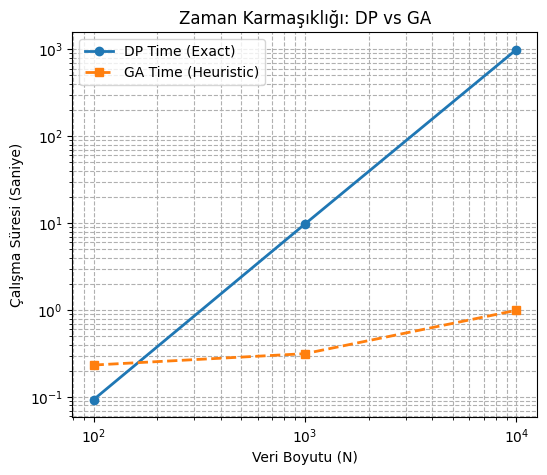
\includegraphics{Unknown.png}}
\caption{DP ve GA Algoritmalarının Zaman Karmaşıklığı Karşılaştırması (Log-Log Ölçek).}
\label{fig:time_complexity}
\end{figure}

\section{Sonuç (Conclusion)}
DP algoritması kesin optimum çözümü bulmakta başarılı olsa da, büyük ölçekli problemlerde (N=10.000) $\approx 990$ saniyelik hesaplama maliyeti ile sistem sınırlarını zorlamıştır. GA ise esnek kısıt yönetimindeki zayıflığına rağmen, büyük veri boyutlarında yalnızca $\approx 1$ saniyede çalışarak zaman açısından muazzam bir avantaj sağlamış, ancak optimum değerden $\%65.12$ feragat etmiştir. Gelecek çalışmalarda, GA'nın geçerli çözüm bulma oranını artırmak için onarım (repair) operatörlerinin entegre edilmesi hedeflenmektedir.

\begin{thebibliography}{00}
\bibitem{b1} F. F. Sakib, J. S. Joy, S. I. Juel and M. M. Hasan, ``Applying Heuristic Algorithms for Solving the 0-1 Knapsack Problem: An Experimental Analysis,'' \textit{2025 4th International Conference on Robotics, Electrical and Signal Processing Techniques (ICREST)}, Dhaka, Bangladesh, 2025, pp. 356-360.

\bibitem{b2} I. Y. CR, A. R, P. T. Ramana, P. Shilpa and J. G, ``Comparative Performance Analysis of Genetic Algorithm Variants on Solving 0/1 Knapsack Problem,'' \textit{2023 IEEE World Conference on Applied Intelligence and Computing (AIC)}, Sonbhadra, India, 2023, pp. 125-130.

\bibitem{b3} G. R. Raidl, ``An improved genetic algorithm for the multiconstrained 0-1 knapsack problem,'' \textit{1998 IEEE International Conference on Evolutionary Computation Proceedings}, Anchorage, AK, USA, 1998, pp. 207-211.
\end{thebibliography}

\end{document}